\documentclass[./main.tex]{subfiles}


\begin{document}
\chapter{Logica e automazione dei problemi di Decisione}

In questo capitolo verranno descritte le nozioni di base necessarie 
per comprendere il lavoro svolto in questa tesi. 
In particolare, verranno introdotti i concetti di logica proposizionale e 
del primo ordine, definita come estensione della prima.
Verrà anche introdotto il problema della decisione, ovvero il problema di stabilire se una data formula è soddisfacibile o meno
e le principali tecniche ad alto livello che vengono utilizzate dai theorem prover moderni per risolvere questo problema.
Nell'ultimo paragrafo del capitolo 
verrà descritto in che modo le formule di logica del 
primo ordine possono essere rappresentate in un formato di file, per poi essere 
processate come input da un theorem prover. 
Lo scopo di questo capitolo è quindi quello di accennare la teoria logica utilizzata nell'implementazione di vampire 
e della procedura di decisione per i Binding-Fragments.
Non è tra gli obbiettivi dare una trattazione esaustiva sulla logica o in generale sulle varie teoria matematiche coinvolte, 
perciò verranno date per scontate nozioni di teoria degli insiemi,
algebra, teoria della computazione e teoria dei linguaggi.



\section{Logica Proposizionale}

La logica proposizionale è un ramo della logica formale che si occupa dello studio e della manipolazione delle proposizioni, 
ovvero dichiarazioni che possono essere classificate come vere o false, ma non entrambe contemporaneamente (Principio di bivalenza).
Essa fornisce un quadro formale per analizzare il ragionamento deduttivo basato su connettivi logici, come "e", "o", e "non".
Questo strumento anche se incluso nella logica del primo ordine,
rimane un pilastro fondamentale per lo studio svolto in questa tesi e quindi è necessario farne un'introduzione indipendente.

% ---------------------- FORMULE ----------------------
\subsection{Formule}
Sia $\Sigma_c = \{c_1, c_2, ...\}$ un insieme di simboli di costante, 
$\Sigma = \{ \land, \lor, \lnot, (, ), \top, \bot\} \cup \Sigma_c$ è detto alfabeto della logica proposizionale. 
%Dato un insieme di simboli $A$, l'insieme $A^*$ è definito come l'insieme delle stringhe finite su $A$.
Con queste premesse si può definire come formule della logica proposizionale il linguaggio $F$ generato dalla
grammatica Context Free seguente:
$$
\varphi  := \top \mid \bot \mid C \mid \lnot \varphi \mid (\varphi \land \varphi) \mid (\varphi \lor \varphi)
$$

Dove $C \in \Sigma_c$ è un simbolo di costante. Con la funzione $const(\gamma) \rightarrow 2^{\Sigma_c}$ si indica la funzione che
associa a ogni formula $\gamma$ l'insieme dei suoi simboli di costante. 
Viene chiamato \textit{Letterale}, ogni simbolo di costante $c$ o la sua negazione $\lnot c$.
Vengono inoltre introdotti i seguenti simboli come abbreviazioni:

\begin{itemize}
    \item $(\gamma \Rightarrow \kappa)$ per $(\lnot \gamma \lor \kappa)$
    \item $(\gamma \Leftrightarrow \kappa)$ per $((\gamma \Rightarrow \kappa) \land (\kappa \Rightarrow \gamma))$
    \item $(\gamma \oplus \kappa)$ per $\lnot(\gamma \Leftrightarrow \kappa)$
\end{itemize}

È possibile rappresentare una qualunque formula attraverso il proprio albero di derivazione. Questo albero 
verrà chiamato in seguito anche \textit{albero sintattico} della formula. Ad esempio, la formula 
$(c_1 \land c_2) \lor \lnot c_3$ può essere rappresentata dal seguente albero sintattico:

\begin{center}
    \begin{tikzpicture}[level distance=1cm,
        level 1/.style={sibling distance=3cm},
        level 2/.style={sibling distance=1.5cm}]
        \node {$\lor$}
          child { node {$\land$}
            child {node {$c_1$}}
            child {node {$c_2$}}
          }
          child { node {$\lnot$}
            child {node {$c_3$}}
          };
    \end{tikzpicture}
\end{center}


La radice dell'albero è detta \textit{connettivo principale} e i sotto alberi della formula vengono dette \textit{sottoformule}.
 Per compattezza, grazie alla proprietà associativa di $\land$ e $\lor$, è possibile omettere le parentesi, es. 
$(c_1 \land (c_2 \land (c_3 \land c_4))) \lor c_5$ può essere scritto come $(c_1 \land c_2 \land c_3 \land c_4) \lor c_5$. 
Allo stesso modo, nell'albero sintattico della formula è possibile compattare le catene di $\land$ e $\lor$ come figli di un unico nodo:

\begin{center}
    \begin{tikzpicture}[level distance=1cm,
        level 1/.style={sibling distance=2.5cm},
        level 2/.style={sibling distance=1cm}]
        \node {$\lor$}
          child { node {$\land$}
            child {node {$c_1$}}
            child {node {$c_2$}}
            child {node {$c_3$}}
            child {node {$c_4$}}
          }
            child { node {$c_5$}};
    \end{tikzpicture}
\end{center}

Questa è una caratteristica molto importante, in quanto non solo permette di risparmiare inchiostro, ma consente di vedere
$\land$ e $\lor$ non più come operatori binari ma come operatori n-ari. A livello implementativo, ciò si traduce in un minor
impatto in memoria, visite all'albero più veloci e algoritmi di manipolazione più semplici. Si consideri ad esempio di voler ricercare la 
foglia più a sinistra nell'albero di derivazione della seguente formula $(( ... (((c_1 \land c_2) \land c_3) \land c_4) \land ... )\land c_n)$.
Senza compattazione, l'algoritmo di ricerca impiegherebbe $O(n)$ operazioni, mentre con la compattazione $O(1)$.

% ---------------------- END FORMULE ----------------------


% ---------------------- Assegnamenti ----------------------

\subsection{Assegnamenti}

Un \textit{assegnamento} è una qualunque funzione $\alpha$ da un 
insieme $C \subseteq \Sigma_c$ nell'insieme $\{1, 0\}$ (o $\{True, False\}$).
$$ \alpha : C \rightarrow \{1, 0\} $$
Un assegnamento $\alpha$ è detto \textit{appropriato}  per una formula $\varphi \in F$ se e solo se $const(\varphi) \subseteq dom(\alpha)$.

Si definisce la relazione binaria di \textit{Soddisfacibilità}: 
$$\models \, \subseteq \{1, 0\}^{C} \times F$$
In modo tale che dato un assegnamento $\alpha$ appropriato a una formula $\varphi$, si dice che $\alpha \models \varphi$ ($\alpha$ soddisfa $\varphi$) 
o anche $\alpha$ è un assegnamento per $\varphi$ o  se e solo se:

\begin{itemize}
  \item Se $\varphi$ è una costante (o $\top$/$\bot$) $c_x$ allora $\alpha \models \varphi$ sse $\alpha(c_x) = 1$
  \item Se $\varphi$ è della forma $\lnot \psi$ (dove $\psi$ è una formula) allora $\alpha \models \varphi$ sse $\alpha \not\models \psi$
  \item Se $\varphi$ è della forma $(\psi \land \chi)$ (con $\psi$ e $\chi$ formule) allora $\alpha \models \varphi$ sse $\alpha \models \psi$ e $\alpha \models \chi$
  \item Se $\varphi$ è della forma $(\psi \lor \chi)$ (con $\psi$ e $\chi$ formule) allora $\alpha \models \varphi$ sse $\alpha \models \psi$ o $\alpha \models \chi$
\end{itemize}

Per convenzione si assume che $\alpha(\top) = 1$ e $\alpha(\bot) = 0$ per ogni assegnamento $\alpha$.
Una \textit{Tautologia} è una formula $\varphi$ tale che per ogni assegnamento $\alpha$ appropriato a $\varphi$, $\alpha \models \varphi$ (in simboli $\models \varphi$).
Una formula è detta soddisfacibile se esiste un assegnamento appropriato che la soddisfa altrimenti è detta insoddisfacibile.
Date due formule $\varphi$ e $\psi$, si dice che $\psi$ è \textit{conseguenza logica} di $\varphi$ (in simboli $\varphi \models \psi$) 
se e solo se per ogni assegnamento $\alpha$ appropriato a entrambe le formule, se $\alpha \models \varphi$ allora $\alpha \models \psi$.
Due formule sono dette \textit{equivalenti} sse $\varphi \models \psi$ e $\psi \models \varphi$ (in simboli $\varphi \equiv \psi$).
Un'importante proprietà è che se $\varphi \models \psi$ allora la formula $\varphi \Rightarrow \psi$ 
è una tautologia ($\models \varphi \Rightarrow \psi$).

Due concetti molto simili a quello di equivalenza e conseguenza logica sono l'\textit{equisoddisfacibilità} e la \textit{soundness}. In pratica, due formule sono sound
se e solo se, se la prima formula è soddisfacibile allora lo è anche la seconda. Due formule sono equisoddisfacibili se e solo se sono sound in entrambe le direzioni. 
Quindi la conseguenza logica implica la soundness ma non il viceversa. Allo stesso modo l'equivalenza
logica implica l'equisoddisfacibilità ma non il viceversa. Si consideri ad esempio le due formule $\varphi = c_1$ e $\psi = \lnot c_1$. Ovviamente non 
può esserci conseguenza logica tra le due formule, ma sono equisoddisfacibili, infatti se $\alpha$ è un assegnamento per $\varphi$ allora è possibile
costruire un assegnamento $\beta$ per $\psi$ tale che $\beta(c_1) = 1-\alpha(c_1)$ e viceversa.

Un'\textit{inferenza} è una qualunque funzione da $F$ in $F$. Un'inferenza è detta \textit{corretta} se conserva la soddisfacibilità, ovvero 
se non può generare una formula insoddisfacibile a partire da una formula soddisfacibile (soundness).

Infine, si definisce \textit{Implicante} di una formula $\varphi$ un insieme $I$ di letterali di $\varphi$ che rendono vera $\varphi$. Cioè, costruendo una
assegnazione $\alpha$ tale che $\alpha \models c$ per ogni letterale $c \in I$, si ha che $\alpha \models \varphi$. In altre parole la formula 
costruita dalla congiunzione di tutti i letterali di $I$ implica logicamente $\varphi$. Spesso con abuso di terminologia gli elementi di $I$ vengono chiamati
anch'essi implicanti, di solito è facile intuire dal contesto se si sta parlando dell'insieme o dei letterali.
È possibile anche costruire un Implicante a partire da una assegnazione. È sufficiente prendere l'insieme dei letterali della formula soddisfatti dall'assegnamento e 
si ottiene così un implicante.

% ---------------------- END Assegnamenti ----------------------

% ---------------------- Forme Normali ----------------------
\subsection{Forme Normali} \label{sec:forme_normali}
Una delle strategie più utilizzate dai dimostratori di teoremi automatici è la \textit{normalizzazione} delle formule. Una \textit{forma normale}
è essenzialmente un sottoinsieme di $F$ che rispetta determinate proprietà. Una \textit{normalizzazione} invece è il processo di trasformazione di una formula
tramite una successione d'inferenze (corrette) in una forma normale.
In questo paragrafo verranno descritte le tre forme normali che sono state utilizzate per il preprocessing
dell'algoritmo. In questo caso, tutte e tre le forme presentate preservano la relazione di equivalenza logica, quindi è sempre possibile
trasformare una formula in un'altra equivalente in uno di questi tre formati. 
La prima e l'ultima ossia le forme NNF e CNF sono le più famose e utilizzate, mentre la seconda, la ENNF, non è abbastanza conosciuta da essere definita standard
e viene utilizzata per bypassare alcuni problemi di efficienza causati dalla CNF grazie all'utilizzo di tecniche di Naming, che però verranno discusse nella prossima sezione.

La prima tra queste è la \textit{NNF} ossia \textit{Negated Normal Form} (Forma normale negata). Una formula è in formato NNF 
sse non contiene connettivi semplificati ($\Rightarrow$, $\Leftrightarrow$, $\oplus$) e la negazione è applicata solo a letterali. La classe di formule 
NNF è generata dalla seguente grammatica:

$$ \eta := \top \mid \bot \mid C \mid \lnot C \mid (\eta \land \eta) \mid (\eta \lor \eta ) $$

Dove $C \in \Sigma_c$ è un simbolo di costante. La normalizzazione di una formula in NNF è un processo semplice che consiste nell'applicare opportunamente 
le regole di De Morgan e le regole di semplificazione dei connettivi.

La seconda forma normale è la \textit{ENNF} ossia \textit{Extended Negated Normal Form} (Forma normale negata estesa). 
Il formato ENNF è essenzialmente una classe più permissiva della NNF, in quanto conserva il vincolo sulla negazione ma 
vieta esclusivamente l'uso di '$\Rightarrow$'. La classe di formule ENNF è generata dalla seguente grammatica:
 
$$ \overline{\eta}  := \top \mid \bot \mid C \mid \lnot C \mid (\overline{\eta} \land \overline{\eta}) \mid (\overline{\eta} \lor \overline{\eta} ) \mid (\overline{\eta} \Leftrightarrow \overline{\eta}) \mid (\overline{\eta} \oplus \overline{\eta}) $$

La terza e ultima forma normale è la \textit{CNF} ossia \textit{Conjunctive Normal Form} (Forma normale congiuntiva). Una formula è in formato CNF
sse è una congiunzione di disgiunzioni di letterali. La classe di formule CNF è generata dalla seguente grammatica:


$$ \zeta := \xi \mid (\xi \land \zeta) $$
$$ \xi := \top \mid \bot \mid C \mid \lnot C \mid (\xi \lor \xi ) $$

La classe CNF è storicamente la più famosa e utilizzata, in quanto è la più semplice da implementare e da manipolare. È possibile vedere le clausole
come insiemi di letterali mentre la formula principale è vista come un insieme di clausole. Ad esempio, la CNF $(c_1 \lor \lnot c_2) \land (c_3)$ può essere rappresentata
in termini insiemistici come $\{\{c_1, \lnot c_2\}, \{c_3\}\}$. 
La clausola vuota $\{\}$ è una clausola speciale che rappresenta la formula $\bot$, viene spesso raffigurata dal simbolo $\square$.
La normalizzazione di una formula in CNF è un processo più complesso rispetto alle altre due forme normali. Non esiste un unica tecnica di normalizzazione, ma
una strategia comune è questa:
\begin{enumerate}
  \item Si trasforma la formula in NNF.
  \item Se la formula è del tipo $\varphi_1 \land ... \land \varphi_n$ allora la struttura principale è già una congiunzione di formule,
   quindi si procede applicando l'algoritmo sulle sottoformule $\varphi_1, ..., \varphi_n$.
  \item Se la formula è del tipo $(\varphi_1 \land \varphi_2) \lor \psi_1$ si applica la proprietà distributiva di $\lor$ su $\land$ in 
  modo da spingere i connettivi $\lor$ il più possibile in profondità. Si ottiene così una formula del tipo
  $(\varphi_1 \lor \psi_1) \land (\varphi_2 \lor \psi_1)$ si procede poi ricorsivamente con il punto 2.
\end{enumerate}

Il processo di generazione delle clausole prende il nome di \textit{clausificazione}.
Questa tecnica di clausificazione nella peggiore delle ipotesi porta a una generazione di un numero di clausole esponenziale 
rispetto alla dimensione della formula originale. Ad esempio la formula $(c_1 \land c_2) \lor (c_3 \land c_4) \lor ... \lor (c_{n-1} \land c_{n})$ 
genera esattamente $2^{n}$ clausole diverse tutte da $n$ letterali.


% ---------------------- END Forme Normali ----------------------

% ---------------------- Naming ----------------------
\subsection{Naming}
Come già accennato il processo di normalizzazione di una formula può portare a una crescita esponenziale del numero di clausole generate.
Si assuma ad esempio di voler clausificare una formula del tipo:

$$ \varphi \lor \psi$$

E che $\varphi$ e $\psi$ generino rispettivamente $n$ e $m$ clausole. Continuando a clausificare con l'algoritmo 
descritto nel paragrafo \ref{sec:forme_normali}, si ottengono $n \cdot m$ clausole. 
Questo perché la continua applicazione della proprietà distributiva porta a una duplicazione considerevole delle sottoformule.
Una possibile tecnica di ottimizzazione è quella del \textit{Naming} anche detto \textit{Renamig}.
In generale per \textit{Naming} si intende una qualunque tecnica di rinomina di letterali o sottoformule.
In questo caso, per \textit{Naming} si intende la rinomina di sottoformule tramite l'aggiunta di un nuovo simbolo di costante.
Per l'esempio precedente si assuma che $c_n$ sia un simbolo di costante non presente nella formula originale.
Applicando il \textit{Naming} si ottiene la seguente formula:

$$ (\varphi \lor c_n) \land (c_n \lor \psi)$$

In questo modo, la clausificazione della formula genera solo $n + m$ clausole al costo dell'aggiunta di un nuovo simbolo di costante.
Un discorso simile vale per formule con la doppia implicazione e lo xor, solo che in questo caso
anche solo la normalizzazione in NNF può portare a una crescita esponenziale del numero di sottoformule.
La trasformazione in NNF e poi in CNF della formula:

$$ ((...((c_1 \Leftrightarrow c_2) \Leftrightarrow c_3) \Leftrightarrow ...) \Leftrightarrow c_n)$$

Porta alla generazione di $2^{n-1}$ clausole. Nell'esempio particolare in cui $n=6$ si ottengono $32$ clausole ma con l'introduzione 
di due nuovi nomie $c_7$ e $c_8$ è possibile ottenere la seguente formula:

$$ (c_7 \Leftrightarrow (((c_1 \Leftrightarrow c_2) \Leftrightarrow c_3) \Leftrightarrow c_4)) $$
$$ \land $$
$$ (c_8 \Leftrightarrow (c_7 \Leftrightarrow c_5)) $$
$$ \land $$
$$ (c_8 \Leftrightarrow c_6) $$

Che genera solo $22$ clausole.
Il processo per stabilire quale sottoformula rinominare è un problema complesso. 
Solitamente stabilisce un numero detto \textit{Threshold} (Soglia) che rappresenta il numero massimo di clausole che si è disposti a generare.
Se una sottoformula genera un numero di clausole maggiore del Threshold, allora viene rinominata. 
Ma anche questo è un discorso non banale e non verrà approfondito oltremodo in questo documento.
In generale la nuova formula generata dal namig è equisoddisfacibile all'originale.

% ---------------------- END Naming ----------------------

\section{Logica del primo ordine}

La logica dei predicati rappresenta un'estensione della logica proposizionale, 
ampliando il suo ambito per trattare in maniera più ricca e dettagliata le relazioni tra gli oggetti 
e le proprietà delle entità coinvolte. Mentre la logica proposizionale si occupa di proposizioni atomiche, 
la logica dei predicati introduce i predicati,
che sono relazioni che sono vere o false a seconda dell'interpretazione e dalle variabili che contengono.
Vengono generalizzati anche i connettivi logici $\land$ e $\lor$ tramite i quantificatori universali e esistenziali $\forall$ e $\exists$
in modo da poter parlare di anche di insiemi di oggetti non finiti.


% ---------------------- Termini ----------------------
\subsection{Termini e Formule} \label{sec:sintassi_fof}
Oltre al solito insieme $\Sigma_c$ di simboli di costante, vengono introdotti tre nuovi insiemi di simboli:
\begin{itemize}
  \item $\Sigma_f = \{f_1, f_2, ...\}$ insieme di simboli di funzione
  \item $\Sigma_p = \{p_1, p_2, ...\}$ insieme di simboli di predicato (o relazione)
  \item $\Sigma_x = \{x_1, x_2, ...\}$ insieme di simboli di variabile
\end{itemize}

Si definisce la funzione $arity : \Sigma_f \cup \Sigma_p \rightarrow \mathbb{N}$ che associa ad ogni simbolo di funzione o predicato la sua arità.
I simboli contenuti in $\Sigma_c \cup \Sigma_f \cup \Sigma_p$ sono detti \textit{simboli non logici} e ogni suo sottoinsieme è detto \textit{tipo}.
Un \textit{termine} è una stringa generata dalla seguente grammatica:

$$ \tau := X \mid C \mid f(\tau_1, ..., \tau_n) $$

Dove $X$ è un simbolo di variabile, $C$ è un simbolo di costante e $f$ è un simbolo di funzione tale che $arity(f) = n$. In altre parole:
\begin{itemize}
  \item Ogni variabile è un termine
  \item Ogni costante è un termine
  \item Se $\tau_1, ..., \tau_n$ sono termini e $f$ è un simbolo di funzione di arità $n$ allora $f(\tau_1, ..., \tau_n)$ è un termine
\end{itemize}

Si indica con $T$ l'insieme di tutti i termini generati dalla grammatica precedente.
Chiameremo \textit{Atomo} tutte le stringhe del tipo $p(\tau_1, ..., \tau_n)$ dove $p$ è un simbolo di relazione
di arità $n$ e $\tau_1, ..., \tau_n$ sono termini.
Si considerano atomi anche tutti i simboli di costante.
Vengono chiamati \textit{Letterali} tutti gli atomi e la loro negazione.
Termini e Letterali sono detti \textit{ground} se non contengono variabili.
Come già visto per le formule proposizionali, è possibile rappresentare un termine o un letterale
attraverso il proprio albero di derivazione. Ad esempio, il letterale $p_1(f(x_1, c_2), c_1)$ può essere rappresentato dal seguente albero sintattico:

\begin{center}
  \begin{tikzpicture}[level distance=1cm,
    level 1/.style={sibling distance=3cm},
    level 2/.style={sibling distance=1.5cm}]
    \node {$p$}
      child { node {$f$}
        child {node {$x_1$}}
        child {node {$c_2$}}
      }
      child { node {$c_1$}};
  \end{tikzpicture}
\end{center}

Come intuibile i sottoalberi di un termine sono detti \textit{sottotermini}. Si assuma di avere due letterali $p_1(c_1, f_1(x_1, c_2))$ e 
$\lnot p_1(f_2(f_1(x_1, c_2), c_2), c_2)$ di volerli rappresentare in un unico grafo. Al posto di creare una foresta con due alberi indipendenti,
è possibile creare un unica struttura condividendo i sottotermini comuni:

\begin{center}
  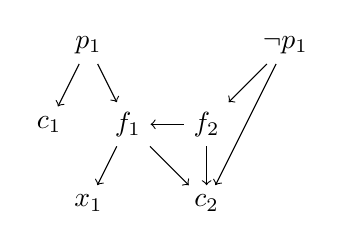
\begin{tikzpicture}[level distance=1cm,
    level 1/.style={sibling distance=3cm},
    level 2/.style={sibling distance=1.5cm}]
    
    \node (p) at (0.5, 0) {$p_1$};
    \node (np) at (3, 0) {$\lnot p_1$};
    \node (f) at (1, -1) {$f_1$};
    \node (g) at (2, -1) {$f_2$};
    \node (x) at (0.5, -2) {$x_1$};
    \node (c1) at (0, -1) {$c_1$};
    \node (c2) at (2, -2) {$c_2$};

    \path [->] (p) edge (f);
    \path [->] (p) edge (c1);

    \path [->] (np) edge (g);
    \path [->] (np) edge (c2);

    \path [->] (f) edge (x);
    \path [->] (f) edge (c2);

    \path [->] (g) edge (f);
    \path [->] (g) edge (c2);

  \end{tikzpicture}
\end{center}

Una struttura del genere è detta \textit{Prfectly Shared} (Perfettamente condivisa). Nella pratica questa
tecnica di condivisione di sottotermini è indispensabile dato che,
anche se a un costo per la creazione e la gestione non indifferente,
permette un risparmio di memoria e di tempo considerevole. Per effettuare ad esempio un controllo 
di uguaglianza tra due sottotermini è sufficiente controllare che le due frecce che partono dai termini padre
puntino allo stesso sottotermine, senza dover visitare l'intera sotto struttura, rendendo così tale operazione a tempo costante.


A questo punto si definisce finalmente le formule della logica del primo ordine. Prendendo come punto di partenza le formule proposizionali,
si definisce alfabeto delle formule del primo ordine l'insieme: 
$\Sigma' = \Sigma \cup \Sigma_f \cup \Sigma_p \cup \Sigma_x \cup \{\forall, \exists\}$ 
e Si definisce come formule del primo ordine il linguaggio $F'$ generato dalla seguente grammatica:

$$ \phi := \top \mid \bot \mid A \mid \lnot \phi \mid (\phi \land \phi) \mid (\phi \lor \phi) \mid \forall x (\phi) \mid \exists x (\phi) $$

Dove $A$ è un atomo e $x$ è un simbolo di variabile. I simboli $\forall$ e $\exists$ sono detti quantificatori universali ed esistenziali.
Una variabile $x$ è detta \textit{vincolata} se è contenuta in una formula del tipo $\forall x (\varphi')$ o $\exists x (\varphi')$ 
altrimenti è detta \textit{libera}. Una formula è detta \textit{enunciato} se non contiene variabili libere. Una formula è detta 
\textit{ground} se tutti i suoi letterali sono ground.

Per comodità di scrittura è possibile raggruppare catene di quantificatori dello stesso tipo. Ad esempio, la formula 
$ \forall x_1 \forall x_2 \forall x_3 \exists x_4 \exists x_5 \forall x_6 \forall x_7 (\phi)$ può essere scritta come 
$\forall x_1 x_2 x_3 \exists x_4 x_5 \forall x_6 x_7 (\phi)$. Così come visto per $\lor$ e $\land$ è possibile vedere
$\forall$ e $\exists$ come operatori n-ari che prendono in input n-1 variabili e una formula.


% ---------------------- END Termini ----------------------

% ---------------------- Unificazione ----------------------
\subsection{Unificazione}
Dato un termine $\tau$ (o un letterale), con la scrittura $\tau[x_k/t]$ si indica il termine (o il letterale) ottenuto sostituendo
tutte le occorrenze della variabile $x_k$ con il termine $t$ in $\tau$. Ad esempio se $\tau = f(x_1, x_2)$ allora $\tau[x_1/c_1] = f(c_1, x_2)$.
Si può estendere questa notazione in modo da poter sostituire più variabili contemporaneamente. 
Si definisce come \textit{sostituzione} una qualunque funzione da variabili a termini.
Dato un termine $\tau$ e una sostituzione $\sigma = \{(x_1, t_1), ..., (x_n, t_n)\}$,
con la scrittura $\tau[x_1/t_1, ..., x_n/t_n]$ oppure $\tau^\sigma$ si indica il termine ottenuto sostituendo \textit{contemporaneamente} 
tutte le occorrenze delle variabili $x_1, ..., x_n$ con i termini $t_1, ..., t_n$ in $\tau$.
Con contemporaneamente si intende che ogni singola sostituzione viene effettuata sul termine originale, 
senza essere influenzata dalle sostituzioni precedenti o successive.
Ad esempio, se $\tau = f(x_1, x_2)$ allora $\tau[x_1/x_2, x_2/x_1] = f(x_2, x_1)$ e non $f(x_1, x_1)$ 
che è invece il risultato dell'applicazione sequenziale delle due regole $\tau[x_1/x_2][x_2/x_1]$.

Dati due termini $\tau_1$ e $\tau_2$ si dice che $\tau_1$ è \textit{più generico} di $\tau_2$ o che $\tau_2$ è \textit{più specifico} di $\tau_1$
se e solo se esiste una sostituzione $\sigma$ tale che $\tau_1^\sigma = \tau_2$.
Se esiste una sostituzione $\sigma$ tale che $\tau_1^\sigma = \tau_2^\sigma$ allora i due termini sono detti \textit{unificabili} e 
la sostituzione $\sigma$ è detta \textit{unificatore} dei due termini.


Date due sostituzioni $\sigma_1$ e $\sigma_2$ si dice che $\sigma_1$ 
è \textit{più generica} di $\sigma_2$ o che $\sigma_2$ è \textit{più specifica} di $\sigma_1$ se e solo se 
per ogni termine $\theta$, $\sigma_2$ è sussunta da $\sigma_1$, 
ossia sse esiste una sostituzione $\theta$ tale che $\tau^{\sigma_2} = {(\tau^{\sigma_1})}^\theta$.
Dati due termini unificabili $\tau_1$ e $\tau_2$ si dice che $\sigma_1$ è un \textit{MGU} (Most General Unifier) di $\tau_1$ e $\tau_2$ 
se è la sostituzione più generica tra tutti gli unificatori dei due termini.


È possibile generalizzare il concetto di unificazione per insiemi di termini, letterali e insiemi di letterali.
Dato un insieme di termini $T$, si dice che $T$ è unificabile se esiste una sostituzione $\sigma$ tale che $\tau_1^\sigma = \tau_2^\sigma$
per ogni coppia di termini $\tau_1, \tau_2 \in T$. In questo caso $\sigma$ è detto unificatore di $T$. 
Due letterali della stessa arità $L_1 = p_1(\tau_1, ..., \tau_n)$ e $L_2 = p_2(\tau_1', ..., \tau_n')$ 
sono unificabili se e solo se esiste una sostituzione che li eguaglia ignorando il simbolo di predicato.
In altre parole sia $f$ una funzione di arità $n$ allora $L_1$ e $L_2$ sono unificabili se e solo se sono unificabili i termini
$f(\tau_1, ..., \tau_n)$ e $f(\tau_1', ..., \tau_n')$.
Letterali di diversa arità non sono mai unificabili.
Un insieme di letterali è unificabile se e solo se esiste una sostituzione che unifica a due a due tutti i letterali dell'insieme.
% Si dirà anche che un insieme di liste di termini $\{\underline{\tau_1}, ..., \underline{\tau_n}\}$ è unificabile 
% se e solo se tutte le liste hanno la stessa lunghezza $n$ e dato un qualunque predicato $p$ $n$-ario l'insieme 
% $\{p(\underline{\tau_1}), ..., p(\underline{\tau_n})\}$ è unificabile.


Un importante risultato è questo:
\newtheorem{proposition}{Proposizione}
\begin{proposition}
  Se due termini non sono unificabili allora vale una delle seguenti affermazioni:
  \begin{enumerate}
    \item I due termini hanno arità diverse
    \item I due termini presentano una function obstruction 
    \item I due termini presentano una variable obstruction
  \end{enumerate}
\end{proposition}

Una function obstruction è una situazione in cui visitando allo stesso modo l'albero sintattico dei termini si incontrano
due simboli di funzione diversi. Ad esempio, i termini $f_1(x_1, f_2(x_2))$ e $f_1(x_1, f_3(x_2))$ non sono unificabili in quanto
presentano una function obstruction, $f_2 \neq f_3$. Una variable obstruction invece è una situazione in cui visitando allo stesso modo
l'albero sintattico dei termini si incontra una variabile $x$ nel primo termine 
e si incontra un sottotermine $t \; (\neq x)$ che contiene $x$ nel secondo termine. Ad esempio i termini $f_1(x_1, f_2(x_2))$ e $f_1(f_2(x_1), x_1)$
non sono unificabili in quanto presentano una variable obstruction, $x_1$ è contenuta in $f_2(x_1)$.


Un noto algoritmo per la ricerca di un MGU di due termini è l'algoritmo di unificazione di \textit{Robinson}. Il collo di bottiglia di questo 
algoritmo è la occurrence-check, ovvero la ricerca di una variable obstruction. Se si assume che i termini in 
input non contengono variabili in comune è possibile ignorare questa situazione. Di seguito viene riportato l'algoritmo di Robinson
senza occurrence-check:

\begin{algorithm}[H]
  \caption{Algoritmo di unificazione di Robinson senza occurrence-check}
  \KwSty{Firma:}{ unify($\tau_1, \tau_2$)}

  \KwIn{$\tau_1, \tau_2$ due termini}
  \KwOut{$\sigma$ un MGU di $\tau_1$ e $\tau_2$ o $\bot$ se non esiste}

  $S :=$ Empty Stack of pair of terms\;
  $\sigma := \text{Empty Substitution}$\;
  \BlankLine
  $S.push(\tau_1, \tau_2)$\;

  \While{S is not Empty}{
    $(\tau_1, \tau_2) := S.pop()$\;
    \BlankLine
    \While{$\tau_1 \: \text{is a variable} \land \tau_1 \neq \tau_1^\sigma$}{
      $\tau_1 := \tau_1^\sigma$\;
    }
    \While{$\tau_2 \: \text{is a variable} \land \tau_2 \neq \tau_2^\sigma$}{
      $\tau_2 := \tau_2^\sigma$\;
    }\
    \BlankLine

    \If{$\tau_1 \neq \tau_2$}{
      \Switch{$\tau_1 \tau_2$}{
        \textbf{case} $\tau_1$ is a variable $x$ and $\tau_2$ is a variabile $y$ $\Rightarrow$ $\sigma := \sigma \cup \{x/y\}$\;
        \textbf{case} $\tau_1$ is a variable $x$ $\Rightarrow$ $\sigma := \sigma \cup \{x/\tau_2\}$\;
        \textbf{case} $\tau_2$ is a variable $y$ $\Rightarrow$ $\sigma := \sigma \cup \{y/\tau_1\}$\;
        \textbf{case} $\tau_1 = f(s_1, ..., s_n)$ and $\tau_2 = f(t_1, ..., t_n)$ $\Rightarrow$ $S.push(s_1, t_1), ..., S.push(s_n, t_n)$\;
        \textbf{case} $\tau_1 = f(s_1, ..., s_n)$ and $\tau_2 = g(t_1, ..., t_m)$ $\Rightarrow$ \Return{$\bot$}\;
      }
    }
  }
  \Return{$\sigma$}\;
\end{algorithm}

% ---------------------- END Unificazione ----------------------


% ---------------------- Semantica ----------------------
\subsection{Semantica} \label{sec:semantica_fof}
Si indica con \textit{tipo} di $\varphi$, l'insieme di tutti i simboli non logici presenti nella formula (costanti, funzioni e predicati).
Si definisce \textit{Modello} di un tipo $\Gamma$ una coppia $\mathcal{M} = (D, I)$ dove $D$ è un insieme non vuoto detto \textit{Dominio} e $I$ è una funzione: 
$I: \Gamma \rightarrow D$ detta d'\textit{Interpretazione} che associa ogni simbolo non logico del tipo a un elemento del dominio in modo tale che per ogni simbolo non logico $s$:

\begin{itemize}
  \item Se $s$ è un simbolo di funzione n-aria allora $I(s)$ è una funzione $n$-aria su $D$: $I(s): D^n \rightarrow D$.
  \item Se $s$ è un simbolo di predicato n-ario allora $I(s)$ è una relazione $n$-aria su $D$: $I(s) \subseteq D^n$.
\end{itemize}

Per l'interpretazioni delle costanti si assume che nel dominio siano presenti almeno due oggetti distinti $\{0, 1\} \in D$:
\begin{itemize}
  \item Se $s$ è un simbolo di costante allora $I(s) \in \{0, 1\}$
  \item Se $s$ è $\top$ allora $I(s) = 1$
  \item Se $s$ è $\bot$ allora $I(s) = 0$
\end{itemize}

Per semplicità di lettura, d'ora in poi l'applicazione della funzione $I$ ad un simbolo $s$ verrà indicata con $s^I$.
Si definisce \textit{Contesto}, una qualunque mappatura $\gamma : \Sigma_x \rightarrow D$ che associa variabili a un elemento del dominio.
Con la scrittura $\gamma[x/t]$ si indica il contesto ottenuto sostituendo il valore della variabile $x$ con l'elemento $t$.
Ad esempio se $\gamma = \{x_1 \rightarrow a, x_2 \rightarrow b\}$ allora $\gamma[x_1/b] = \{x_1 \rightarrow b, x_2 \rightarrow b\}$.
Per l'applicazione di un contesto a una variabile si utilizza la stessa notazione usata per le funzioni, ovvero $\gamma(x)$.
Per l'esempio precedente $\gamma(x_1) = a$, $\gamma(x_2) = b$ e $\gamma[x_1/b](x_1) = b$.
Se una variabile $x$ non è presente nel contesto allora si assume che $\gamma(x) = x$.
Si definisce l'interpretazione di un termine o predicato $\tau$ nel contesto $\gamma$ secondo l'interpretazione $I$:

\begin{itemize}
  \item Se $\tau$ è una variabile $x$ allora $\tau^I_\gamma = \gamma(x)$
  \item Se $\tau$ è una costante $c$ allora $\tau^I_\gamma = c^I$ (Le costanti non dipendono dal contesto)
  \item Se $\tau$ è una funzione $f(\tau_1, ..., \tau_n)$ allora $\tau^I_\gamma = f^I({\tau_1}^I_\gamma, ..., {\tau_n}^I_\gamma)$
  \item se $\tau$ è un predicato $p(\tau_1, ..., \tau_n)$ allora $\tau^I_\gamma = p^I({\tau_1}^I_\gamma, ..., {\tau_n}^I_\gamma)$
\end{itemize}


Data una formula del primo ordine $\varphi$ si dice che il modello $\mathcal{M}$ è appropriato per la formula $\varphi$ se e solo se il tipo della formula è contenuto nel tipo del modello.
Un modello appropriato $\mathcal{M}$ soddisfa una formula $\varphi$ nel contesto $\gamma$ se e solo se:
\begin{itemize}
  \item Se $\varphi$ è una costante $c$ (o $\top$/$\bot$) allora $\mathcal{M}, \gamma \models c$ se e solo se $c^I = 1$
  \item Se $\varphi$ è della forma $\lnot \psi$ (dove $\psi$ è una formula) allora $\mathcal{M}, \gamma \models \varphi$ se e solo se $\mathcal{M}, \gamma \not\models \psi$
  \item Se $\varphi$ è della forma $(\psi \land \chi)$ (con $\psi$ e $\chi$ formule) allora $\mathcal{M}, \gamma \models \varphi$ se e solo se $\mathcal{M}, \gamma \models \psi$ e $\mathcal{M}, \gamma \models \chi$
  \item Se $\varphi$ è della forma $(\psi \lor \chi)$ (con $\psi$ e $\chi$ formule) allora $\mathcal{M}, \gamma \models \varphi$ se e solo se $\mathcal{M}, \gamma \models \psi$ o $\mathcal{M}, \gamma \models \chi$
  \item Se $\varphi$ è della forma $\forall x (\psi)$ (dove $\psi$ è una formula) allora $\mathcal{M}, \gamma \models \varphi$
   se e solo se per ogni elemento $m \in D$ vale $\mathcal{M}, \gamma[x/m] \models \psi$
  \item Se $\varphi$ è della forma $\exists x (\psi)$ (dove $\psi$ è una formula) allora $\mathcal{M}, \gamma \models \varphi$ se e solo se
    esiste un elemento $m \in D$ tale che $\mathcal{M}, \gamma[x/m] \models \psi$
  \item Infine se $\varphi$ è un letterale $p(\tau_1, ..., \tau_n)$ allora $\mathcal{M}, \gamma \models \varphi$ se e solo se $p^I({\tau_1}^I_\gamma, ..., {\tau_n}^I_\gamma)$
\end{itemize}

Data una formula $\varphi$ si dice che un modello $\mathcal{M}$ soddisfa $\varphi$ o anche che $\mathcal{M}$ 
è un modello di $\varphi$ se e solo se $\mathcal{M}$ è appropriato per $\varphi$ e $\mathcal{M}, \gamma \models \varphi$ per ogni contesto $\gamma$,
in notazione $\mathcal{M} \models \varphi$. Una formula è detta \textit{soddisfacibile} se esiste un modello che la soddisfa.
Una formula è detta \textit{valida} se ogni modello la soddisfa.
La relazione di conseguenza logica, equivalenza, equisoddisfacibilità e soundness sono definite in modo analogo alla logica proposizionale.


Così come è stata posta questa semantica nessuna formula con variabili libere può avere un modello.
Ad esempio se si considera una formula $\varphi$ con una variabile libera $x$ e si considera un modello $\mathcal{M}$ appropriato per $\varphi$,
è sufficiente prendere un contesto vuoto $\gamma = \{\}$ per ottenere $\mathcal{M}, \gamma \not\models \varphi$.
Per aggirare questa limitazione si estende la definizione di soddisfacibilità per formule con variabili libere.
Dato un modello $\mathcal{M}$ appropriato ad una formula $\varphi$ si dice che $\mathcal{M}$ soddisfa $\varphi$ se e solo se
\begin{itemize}
  \item Se la formula non contiene variabili libere allora la definizione di soddisfacibilità rimane invariata.
  \item Se $\varphi$ contiene variabili libere allora $\mathcal{M} \models \varphi$ se e solo se
  per ogni contesto $\gamma$ che contiene tutte le variabili libere di $\varphi$ vale $\mathcal{M}, \gamma \models \varphi$.
\end{itemize}

Con questa modifica non vi è differenza nel significato tra enunciati del tipo $\forall x (\varphi)$ e formule $\varphi$,
quindi da questo momento in poi ogni variabile libera presente in una formula verrà considerata come vincolata da un quantificatore universale posto all'inizio della formula.

Un'altra osservazione interessante è che se nella formula sono presenti esclusivamente costanti e simboli logici allora il modello si comporta 
esattamente come un'assegnazione proposizionale. È possibile estendere questa considerazione anche alle formule ground, ovvero formule senza variabili.
Infatti se ogni predicato ground viene sostituito da un nuovo simbolo di costante allora la formula proposizionale risultante si comporterà, in termini di soddisfacibilità,
esattamente come la formula originale. Ad esempio la formula ground $(p_1(c_1) \lor p_2(c_2, f_1(c_1))) \land \lnot p_1(c_1) \land c_2$ 
è esattamente equivalente alla formula proposizionale $(c_3 \lor c_4) \land \lnot c_3 \land c_2$, nel senso che per ogni assegnamento proposizionale per la seconda formula
esiste un modello per la prima e viceversa.

% ---------------------- END Semantica ----------------------

% ---------------------- Skolemizzazione e Forme Normali  ----------------------
\subsection{Skolemizzazione e Forme Normali}
In questo paragrafo verrà descritta una procedura fondamentale per la dimostrazione automatica di teoremi, la \textit{Skolemizzazione}. Varrà inoltre introdotta
una nuova forma normale chiamata \textit{PNF} e verranno
estese le forme normali descritte nel paragrafo della logica proposizionale per adattarle alla logica del primo ordine.


La definizione per le forme ENNF e NNF per la logica del primo ordine è pressoché identica a quella della logica proposizionale.
Come per la logica proposizionale, la trasformazione di una formula in ENNF/NNF preserva la relazione di conseguenza logica ed è sempre
possibile trasformare una formula in una equivalente in ENNF/NNF. 
Il calcolo per la normalizzazione viene effettuato allo stesso modo ma con l'aggiunta di due regole per la negazione dei quantificatori:

$$ \lnot \forall x (\varphi) \rightarrow \exists x (\lnot \varphi) $$
$$ \lnot \exists x (\varphi) \rightarrow \forall x (\lnot \varphi) $$


Chiameremo \textit{prefisso di quantificatori} una lista di quantificatori (es. $\forall x_1 \forall x_2 \exists x_3$). 
Un prefisso viene detto \textit{universale} se è composto esclusivamente da quantificatori universali e viene detto \textit{esistenziali} 
se è composto esclusivamente da quantificatori esistenziali. Una formula è in formato PNF (Prenex Normal Form) se tutti e soli 
i quantificatori si trovano all'inizio della formula. La classe di formule PNF è generata dalla seguente grammatica:

$$ P_0 := \rho(P) $$
$$ P := \top \mid \bot \mid A \mid \lnot P \mid (P \land P) \mid (P \lor P) $$

Dove $\rho$ è un prefisso di quantificatori e $A$ è un atomo.
La parte della formula generata dalla seconda regola viene spesso chiamata \textit{matrice}.
È sempre possibile normalizzare una formula in PNF, è un processo sound, ma non è sempre possibile mantenere la relazione di conseguenza logica.


La skolemizzazione è una procedura che permette di eliminare i quantificatori esistenziali da una formula. 
Sia $\rho$ un prefisso di quantificatori qualunque, la funzione $sk : F' \rightarrow F'$ può essere descritta in questo modo:

\begin{itemize}
  \item Se la formula è del tipo $\exists x(\rho \phi)$ allora $sk$ rimuove il primo quantificatore esistenziale e sostituisce 
  la variabile $x$ all'interno della formula con una nuova costante $c_{n+1}$, dove $n$ è il massimo indice di costante presente nella formula.

  \item Se la formula è del tipo $\forall x_k ... x_{k+m-1} \exists x_{k+m} (\rho \phi)$ allora $sk$ rimuove 
  il primo quantificatore esistenziale e sostituisce la variabile $x_{k+m}$ all'interno della formula con una nuova funzione 
  $f_{n+1}(x_k, ... , x_{k+m-1})$
  $m-1$-aria, dove $n$ è il massimo indice di funzione presente nella formula.
\end{itemize}

Applicando la funzione $sk$ tante volte quanto il numero di quantificatori esistenziali presenti nella formula si ottiene una formula 
senza quantificatori esistenziali. Anche la skolemizzazione è un processo sound, ma non è detto che preservi la conseguenza logica.



Combinando le tecniche apprese finora è possibile definire una procedura di normalizzazione che permette di trasformare una formula del primo ordine
in formato CNF. Le formule CNF per il primo ordine sono definite come segue:

$$ \zeta_0 := \rho(\zeta_1) $$
$$ \zeta_1 := \xi \mid (\xi \land \zeta_1) $$
$$ \xi := \top \mid \bot \mid L \mid (\xi \lor \xi ) $$

Dove $\rho$ è un prefisso di quantificatori universale e $L$ un letterale. Per ottenere una formula CNF è sufficiente:

\begin{enumerate}
  \item Normalizzare la formula in NNF
  \item Normalizzare la formula in PNF
  \item Skolemizzare la formula
  \item Applicare lo stesso algoritmo di clausificazione descritto per la logica proposizionale sulla matrice della formula
\end{enumerate}

Visto le tecniche applicate il processo di clausificazione per la logica del primo ordine è sound ma non preserva la conseguenza logica.
Dato che in una formula CNF tutte le variabili sono universalmente quantificate per brevità è possibile omettere il prefisso di quantificatori.
Ad esempio, la formula CNF $\forall x_1 x_2 x_3 x_4 (\lnot p_1(x_1) \lor p_2(x_2) \lor p_3(x_3)) \land (\lnot p_4(x_4))$ può essere scritta come
$(\lnot p_1(x_1) \lor p_2(x_2) \lor p_3(x_3)) \land (\lnot p_4(x_4))$ e quindi rappresentata
in forma insiemistica come $\{\{\lnot p_1(x_1), p_2(x_2), p_3(x_3)\}, \{\lnot p_4(x_4)\}\}$.
Un'osservazione interessante è che visto che tutte le variabili sono universalmente quantificate, è possibile rinominare le variabili di clausole diverse senza
cambiare il significato della formula. È quindi possibile normalizzare le clausole in modo tale che ogni coppia di clausole contenga variabili diverse.
Un caso d'uso tipico è quello di voler unificare due letterali di due clausole diverse. Con l'assunzione che le variabili siano tutte diverse è possibile
applicare l'algoritmo di unificazione senza occurrence-check visto nel capitolo sull'Unificazione.

% ---------------------- END Skolemizzazione e Forme Normali ----------------------


\section{Soddisfacibilità e Validità} \label{sec:sat_val}
Nei precedenti capitoli si è data la definizione di soddisfacibilità e validità per formule proposizionali e del primo ordine.
In questa sezione verrà approfondito il discorso e verranno introdotte alcune nozioni fondamentali per 
capire il funzionamento di un \textit{ATP system} (Automatic Theorem Prover), nonché 
per capire le motivazioni che hanno spinto la creazione di sistemi ATP e i vincoli teorici con cui si devono confrontare.


Il problema della soddisfacibilità/validità è il problema di determinare 
se una formula è soddisfacibile/valida o meno (Una tautologia nel caso della logica proposizionale).
Sorge spontanea la domanda: È possibile creare una procedura che risolva questo problema?
% La risposta è molto complessa e ha tenuto occupati logici e matematici per molti anni.

In primo luogo è bene specificare che il problema della validità è riducibile al problema della soddisfacibilità.
Si immagini di voler dimostrare che una formula $\varphi = (A_1 \land ... \land A_n) \Rightarrow C$ è valida.
Nel caso fosse valida allora la sua negazione $A_1 \land ... \land A_n \land \lnot C$ sarebbe insoddisfacibile.
Nel caso $\lnot \varphi$ fosse soddisfacibile allora esisterebbe
 un modello $\mathcal{M}$ tale che $\mathcal{M} \models \lnot \varphi$ che quindi per definizione 
$\mathcal{M} \not\models \varphi$. In tal caso $\varphi$ non è valida.
In altre parole se un'implicazione è vera allora non è possibile che le premesse siano vere e la conclusione falsa.
Tecniche dimostrative del genere sono dette di \textit{Refutazione} o prove per \textit{Assurdo}.
Esistono anche altre tecniche dimostrative ma la quasi totalità degli ATP si basano sulla refutazione.


Nel caso della logica proposizionale la risposta alla domanda precedente è affermativa, 
anche se il problema è stato dimostrato essere \textit{NP-completo}. 
Esistono vari algoritmi che risolvono il problema,
il più semplice, basato su tavole di verità consiste in un algoritmo 
brute-force che prova tutte le possibili assegnazioni di verità,  
data una formula proposizionale di $n$ costanti esistono al massimo $2^n$ possibili assegnazioni 
quindi è garantito che l'algoritmo termini e dia una risposta corretta.
Un altro dei più famosi è l'algoritmo di Davis-Putnam basato sulla \textit{risoluzione} ma 
tale tecnica verrà approfondita nella sezione dedicata \ref{sec:resolution}.
Nel caso della logica del primo ordine la risposta è più complessa e la strada per arrivarci è lunga e a volte può sembrare anche contorta.


Agli inizi del 900' il famoso matematico David Hilbert pubblicò un articolo in cui elencava 23 problemi matematici, all'epoca aperti,
che avrebbero dovuto guidare la ricerca matematica del secolo successivo. Il secondo problema di Hilbert era il seguente:

\begin{displayquote}
  \textit{È possibile dimostrare la coerenza dell'insieme degli assiomi dell'aritmica?}
\end{displayquote}

La domanda di Hilbert si riferisce al sistema di assiomi dell'aritmetica proposti nei tre volumi di \textit{Principia Mathematica}
di Bertrand Russell e Alfred North Whitehead.
L'indagine del problema portò il suo risolutore, il logico Kurt Gödel, alla scoperta di due importanti risultati.

Il primo risultato, detto \textit{Primo teorema di incompletezza} afferma che:

\begin{displayquote}
  \textit{In ogni sistema formale consistente che contiene un'aritmetica elementare, esiste una formula che non è dimostrabile in quel sistema.}
\end{displayquote}

Il secondo risultato, detto \textit{Secondo teorema di incompletezza} afferma che:

\begin{displayquote}
  \textit{Se un sistema formale consistente contiene un'aritmetica elementare, allora non può dimostrare la propria coerenza.}
\end{displayquote}

Per capire il senso dei due teoremi è necessario introdurre, anche se in maniera informale, i concetti di \textit{Teoria}, \textit{Teorema} e \textit{Sistema formale}.
Un sistema formale è l'unione di questi quattro elementi:

\begin{itemize}
  \item Un alfabeto di simboli.
  \item Delle regole per la generazione di stringhe dette formule.
  \item Un insieme di assiomi.
  \item Un insieme di regole sintattiche dette d'inferenza che associano formule ad altre formule.
\end{itemize}

Un \textit{Teorema} è un assioma o una qualunque formula che può essere ottenuta applicando un numero finito di volte le regole d'inferenza agli assiomi.
Una derivazione sintattica di questo tipo è detta \textit{Dimostrazione} e si indica con $ A_1, ..., A_n \vdash C$
dove $A_1, ..., A_n$ sono gli assiomi e $C$ è la formula derivata detta \textit{congettura}.
Per coerenza si intende la proprietà che il sistema non possa dimostrare una contraddizione,
ad esempio una formula del tipo $\psi \land \lnot \psi$.
Una \textit{Teoria} è un insieme di formule che rispetta le seguenti proprietà:

\begin{enumerate}
  \item $\{A_1, ..., A_n\} \subseteq T$ (Contiene gli assiomi).
  \item Se $A_1, ..., A_n \vdash C$ allora $C \in T$ (Ogni formula derivabile dagli assiomi è nella teoria).
\end{enumerate}

Anche tutto quello che si è visto finora sulla logica è possibile vederlo come un sistema formale.
Si prendano ad esempio come assiomi le formule proposizionali $\{c_1, c_1 \Rightarrow c_2\}$ e come regola d'inferenza
il \textit{Modus ponens}: $[\varphi, \varphi \Rightarrow \psi] \vdash \psi$. Si ottiene che la formula 
$c_2$ è derivabile tramite gli assiomi e le regole d'inferenza.
La teoria sarà composta dalle sole formule: $\{c_1, c_1 \Rightarrow c_2, c_2\}$.
% Un sistema del genere è coerente e tutte le sue inferenze sono \textit{corrette} ma non è \textit{completo}.
% La correttezza e la completezza sono due 


Tornando ai \textit{Principia Mathematica} (\textit{PM}), per riferirsi al sistema formale che vi è contenuto si utilizzerà
la notazione $\vdash_{PM} \varphi$ per indicare che la formula $\varphi$ è dimostrabile nel sistema formale \textit{PM} tramite i suoi assiomi
e le sue regole di derivazione. La tesi di Gödel si basa sulla costruzione di una codifica delle formule e delle dimostrazioni
di PM nello stesso linguaggio formale PM. 
Ogni formula $\varphi$ viene quindi mappata in un numero naturale $\ulcorner  \varphi \urcorner $.
In particolare riesce a formalizzare i predicati:
\begin{itemize}
  \item $Proof(x, y)$ che è vero se e solo se $x$ è la codifica di una dimostrazione di una formula codificata in $y$.
  \item $Thm(x)$ che è vero sse esiste $y\in \mathbb{N} : Proof(y, x)$
  \item $Cons$ che è vero sse il sistema è consistente. Si può anche dire che $Cons$ è vero sse $\lnot Thm(\ulcorner 0 = 1 \urcorner)$
\end{itemize}


Il cuore dei teoremi è una formula $\gamma$, chiamato \textit{enunciato gödeliano},
che afferma di non essere dimostrabile in PM:

$$\gamma := \gamma \Leftrightarrow \lnot Thm(\ulcorner \gamma \urcorner)$$

Il primo teorema di incompletezza si può quindi riformulare in questo modo:
\begin{enumerate}
  \item[1.] Se PM (o un sistema simile) è coerente allora $\nvdash_{PM} \gamma$ e $\nvdash_{PM} \lnot\gamma$
\end{enumerate}

Il secondo teorema di incompletezza si può riformulare in questo modo:

\begin{enumerate}
  \item[2.] Se PM (o un sistema simile) è coerente allora $\nvdash_{PM} Cons$
\end{enumerate}

Si potrebbe fare un discorso molto lungo su cosa significhi \textit{'un sistema simile a PM'} ma 
ciò richiederebbe una dettagliata esplorazione delle dimostrazioni dei teoremi di
Gödel e un approfondimento nella Teoria della \textit{Computabilità}. Tuttavia, eviteremo di approfondire ulteriormente su questi argomenti.
Non si approfondirà nemmeno il discorso sulla verità del predicato godeliano, verrà piuttosto lasciato 
ai filosofi che, in relazione al paradosso del mentitore, dibattono sulla questione da oltre 2000 anni.

In sintesi i teoremi di Gödel minano l'efficacia del lato sintattico di un sistema formale per dimostrare la verità di una formula
ma non cita in nessun modo il lato semantico. Non è detto quindi che non sia possibile dimostrare la verità di una formula indecidibile
utilizzando metodi semantici. Si prenda ad esempio il gioco del \textit{MU} dal libro \textit{Gödel, Escher, Bach} di Douglas Hofstadter.

A chiudere il cerchio tra sistemi formali, aritmetica e logica arriva in aiuto il teorema di Church sull'indecidibilità 
della logica del primo ordine:

\newtheorem{theorem}{Teorema di Church}
\begin{theorem}
  La logica del primo ordine è indecidibile.
\end{theorem}

Il teorema di Church afferma che non esiste un algoritmo che, dato un qualunque enunciato $\varphi$ di una qualunque teoria $T$,
determini se $\varphi$ è dimostrabile in $T$.
La prova si basa sull'applicazione del primo teorema di incompletezza di Gödel al sistema formale \textit{Q}
creato dal logico Raphael Robinson. 
\textit{Q} è un sistema formale che contiene un'aritmetica elementare descritta da un numero finito di assiomi.
Si assuma che $\{q_1, ..., q_n\}$ siano gli assiomi di \textit{Q} e $\varphi$ una qualunque formula.
Se esistesse una procedura di decisione per la logica allora varrebbe:

$$ q_1, ..., q_n \vdash \varphi \text{ se e solo se } \vdash (q_1 \land ... \land q_n) \Rightarrow \varphi$$

Quindi esisterebbe una procedura di decisione anche per \textit{Q},
ma in \textit{Q} vale il primo teorema di Gödel e quindi si giunge a una contraddizione visto che 
si potrebbe provare il predicato godeliano, $\vdash_{Q} \gamma$ o $\vdash_Q \lnot\gamma$.
Ciò discende anche dal fatto che il predicato $Thm$ è \textit{parzialmente calcolabile} ma non \textit{calcolabile},
di conseguenza l'insieme che ha come funzione caratteristica $Thm$ è \textit{ricorsivamente enumerabile} ma non \textit{ricorsivo}.
Quindi si può concludere dicendo che la logica del primo ordine è semidecidibile ma non decidibile.


Il teorema di Church ha delle importanti conseguenze sui sistemi di dimostrazione automatica.
Un ATP infatti può essere visto come un algoritmo di manipolazione sintattica che cerca di dimostrare la validità di una formula
tramite un sistema di inferenze,
ma il teorema di Church afferma che, per quanto sofisticato, esisteranno sempre degli input per cui l'algoritmo non terminerà.
Questa limitazione rappresenta una barriera fondamentale nell'ambito della dimostrazione automatica 
e sottolinea la necessità di considerare approcci misti o raffinamenti nelle strategie di dimostrazione.

\section{Resolution} \label{sec:resolution}
\textit{Resolution} o \textit{Risoluzione} è una regola d'inferenza per logica proposizionale e del primo ordine.
La regola per la logica proposizionale è la seguente:

$$ \frac{\{L\} \cup C_1, \{\lnot L\} \cup C_1}{C_1 \cup C_2} $$

Dove $C_1$ e $C_2$ sono clausole in notazione insiemistica e $L$ è un letterale. 
La regola afferma che se si hanno due clausole dove una contiene un letterale e l'altra la sua negazione allora è possibile
ottenere una nuova clausola che è l'unione delle due clausole senza il letterale e la sua negazione.
Resolution è un'inferenza preserva la conseguenza logica e quindi è corretta. 
Con il nome Resolution spesso ci si riferisce anche ad una classe di algoritmi che sfrutta questa regola come inferenza principale 
per risolvere il problema della soddisfacibilità.
Un famoso esempio di algoritmo per la logica proposizionale basato su Resolution è l'algoritmo di Davis-Putnam anche chiamato \textit{DPP} (Davis-Putnam-Procedure).
La DPP in sintesi procede in questo modo:

\begin{enumerate}
  \item Si trasforma la formula una CNF equivalente
  \item Si eliminano le clausole tautologiche
  (Quelle che contengono sia un letterale che la sua negazione $l \lor \lnot l$).
  \item Si sceglie un qualunque letterale $L$ da una qualunque clausola nella formula $\phi$ ottenuta nel punto precedente.
  \item Si calcolano gli insiemi $S = \{C \in \phi \mid l \notin C \text{ e } \lnot l \notin C\}$ e $T = \phi \setminus S$.
  \item Si calcola l'insieme 
  $R = \{(C_1 \setminus \{L\}) \cup (C_2 \setminus \{\lnot L\}) \mid C_1, C_2 \in T \text{ e } L \in C_1 \text{ e } \lnot L \in C_2\}$, 
  detto dei risolventi, applicando la regola di Resolution.
  \item Si riapplica la procedura dal punto 2. con la nuova formula $\phi' = S \cup R$ finchè o $\phi' = \{\}$
  o $\phi'$ contiene una clausola vuota.
\end{enumerate}

Se l'algoritmo termina con una clausola vuota vuol dire che nel passo precedente la formula conteneva due clausole del tipo $L \land \lnot L$,
quindi la formula originale è insoddisfacibile. Se l'algoritmo termina con $\phi' = \{\}$ allora la formula originale è soddisfacibile.
L'algoritmo seppur corretto è molto inefficiente e non viene utilizzato nella pratica, 
ma è stato il primo basato su Resolution per il problema della soddisfacibilità. 
I SAT solver (programmi che risolvono il problema della soddisfacibilità) si basano su tecniche più raffinate e spesso non sono bassati su Resolution.
Un esempio è l'algoritmo \textit{DPLL} (Davis-Putnam-Logemann-Loveland) che si basa sulle tecniche di \textit{unit propagation} e \textit{pure literal elimination}.


Per la logica del primo ordine, come al solito, il discorso è più complesso.
I primi tentativi di creare un algoritmo per determinare la soddisfacibilità di una formula del primo ordine si
devono ai risultati teorici dei logici 
Skolem, J. Herbrand e R. Robinson. 
I risultati di Herbrand permettono di 'ridurre' il problema della soddisfacibilità di formule universalmente quantificate
al problema della soddisfacibilità di una formula proposizionale. La strategia si basa sulla creazione di un modello 
il quale dominio, detto universo di Herbrand, è generato da tutti i termini ground ottenibili dai termini della formula originale.
L'universo di Herbrand è un insieme finito (se la formula non contiene funzioni) o infinito numerabile. Il secondo passo è 
chiamato istanziazione ground e consiste nel sostituire tutte le variabili con un sottoinsieme finito di elementi dell'universo di Herbrand.
Si ottiene così una formula ground che, come descritto in \ref{sec:semantica_fof}, può essere trasformata in una formula proposizionale e risolta da un Sat Solver. 
Se il Sat solver trova un'assegnazione che soddisfa la formula allora si sceglie un altro sottoinsieme finito diverso dal precedente dell'universo di Herbrand 
e si ripete il procedimento. Se il Sat solver non trova un'assegnazione allora la formula originale è insoddisfacibile.
Se si verificano tutti i sottoinsiemi finiti dell'universo di Herbrand senza trovare formule insoddisfacibili allora la formula originale è soddisfacibile.

È chiaro che la strategia di Herbrand è più un risultato teorico che un metodo pratico.
L'unico caso in cui è garantita la terminazione è quando la formula non contiene funzioni
e quindi l'universo di Herbrand è finito, così come il numero di tutti i sui sottoinsiemi.
I primi algoritmi utilizzabili nella pratica iniziarono a nascere dopo che Robinson introdusse la regola di risoluzione per la logica del primo ordine:

$$ \frac{\{L(\tau_1, ..., \tau_n)\} \cup C_1, \{\lnot L(\omega_1, ..., \omega_n)\} \cup C_1}{(C_1 \cup C_2)^\sigma} $$

Dove $\sigma$ è un unificatore dei due letterali $L(\tau_1, ..., \tau_n)$ e $L(\omega_1, ..., \omega_n)$ e $C_1, C_2$ sono clausole.
Anche per la logica del primo ordine la regola di risoluzione è corretta e preserva la conseguenza logica.
Da qui vi è un punto di svolta nello sviluppo degli ATP.
Il primo ATP ad alte prestazioni basato su Resolution per la logica del primo ordine fu \textit{Otter} sviluppato da William McCune.
Otter fa parte di una classe di theorem prover basati sulla \textit{Saturazione}.
La saturazione è una tecnica concettualmente molto semplice che consiste nel generare 
tutte le clausole possibili a partire da un insieme di clausole iniziali.
Se la formula è insoddisfacibile allora prima o poi verrà generata una clausola vuota.
Se la formula è soddisfacibile allora vi sono due casi possibili.
Nel primo caso l'algoritmo genera tutte le clausole generabili (satura il sistema) e l'algoritmo termina.
Nel secondo caso il numero di clausole generabili dal sistema iniziale non è un numero finito.
In tal caso o l'algoritmo capisce che alcune aree di ricerca non porteranno mai alla generazione 
di una clausola vuota e quindi termina,
oppure, nell'ipotesi peggiore, l'algoritmo non termina mai rimanendo in un loop infinito.
Quest'ultima è una conseguenza inevitabile dei teoremi di Church e Gödel.
Una descrizione più dettagliata di Otter verrà data nel capitolo \ref{chap:vampire} sull'implementazione di Vampire.




\section{Il formato TPTP}
In questa sezione verrà descritto il formato TPTP (Thousands of Problems for Theorem Provers) 
per la rappresentazione di problemi di logica del primo ordine.
TPTP è una nota libreria di problemi utilizzata per testare e valutare diversi ATP systems (Automatic Theorem Prover).
TPTP fornisce diversi formati per la rappresentazione dei problemi,
in questa sezione ci si soffermerà sui formati \textit{CNF} (Clausal Normal Form) e \textit{FOF} (First Order Formula).


La traduzione dei predicati, termini e variabili è la stessa sia per il formato CNF che per il formato FOF.
Ogni variabile è rappresentata da una stringa alfanumerica Maiuscola. 
Simboli di funzione, predicato e costanti sono tutti rappresentati senza distinzione da stringhe alfanumeriche minuscole.
Le regole della grammatica della generazione dei termini è esattamente la stessa vista nel paragrafo \ref{sec:sintassi_fof}.
Per esempio il predicato $p_1(f_1(x_1), x_2, c_1)$ 
può essere rappresentato come \texttt{p1(f1(X1), X2, c1)} o anche \texttt{pred(fun(VAR\_A), VAR\_B, costante)}.


Per la traduzione dei simboli logici si utilizza la seguente mappatura:

\begin{table}[H]
  \centering
  \begin{tabular}{|c|c|}
    \hline
    \textbf{Simbolo} & \textbf{Traduzione} \\
    \hline
    $\top$ & \texttt{\$true} \\
    $\bot$ & \texttt{\$false} \\
    $\lnot$ & \texttt{\~} \\
    $\land$ & \texttt{\&} \\
    $\lor$ & \texttt{|} \\
    $\Rightarrow$ & \texttt{=>} \\
    $\Leftrightarrow$ & \texttt{<=>} \\
    $\oplus$ & \texttt{\url{<~>}} \\
    $\forall$ & \texttt{!} \\
    $\exists$ & \texttt{?} \\
    \hline
  \end{tabular}
  \caption{Traduzione dei simboli logici}
  \label{tab:traduzione_simboli_logici}
\end{table}


Anche le regole per la generazione delle formule sono le stesse viste nella sezione \ref{sec:sintassi_fof},
con l'unica differenza che i simboli logici vengono tradotti secondo la tabella \ref{tab:traduzione_simboli_logici}.
Le parentesi '(' e ')' possono essere omesse e in tal caso si segue il seguente ordine di valutazione dei simboli:
\texttt{!}, \texttt{?}, \texttt{\textasciitilde}, \texttt{\&}, \texttt{|}, \texttt{<=>}, \texttt{=>}, \texttt{\url{<~>}}.
Dopo un quantificatore (\texttt{!}/\texttt{?}) è necessaria la lista delle variabili quantificate racchiuse tra parentesi quadre '[' e ']' 
seguite da ':' e la formula quantificata.
Per esempio la formula $\forall x_1 x_2 \exists x_3 (p_1(x_1) \lor p_2(x_2) \lor p_3(x_3))$ viene 
rappresentata come \texttt{![X1, X2] : (?[X3] : (p1(X1) | p2(X2) | p3(X3)))}.
Se non presenti quantificatori nella formula le variabili libere vengono considerate quantificate universalmente.


Il formato FOF prevede una lista di assiomi seguiti da una congettura. 
Il formato cambia a seconda della domanda che si vuole porre all'ATP.
Data una lista di assiomi $A_1, ..., A_n$ e una congettura $C$:

\begin{itemize}
  \item Se si da in input la lista di assiomi $A_1, ..., A_n$ l'ATP cerca di determinare la Soddisfacibilità della formula $A_1 \land ... \land A_n$.
  \item Se vengono dati sia gli assiomi che la congettura l'ATP cerca di determinare se $A_1 \land ... \land A_n \Rightarrow C$ è valida.
  \item Se invece viene data solo la congettura l'ATP cerca di determinare se $C$ è valida.
\end{itemize}

Il formato per inserire un assioma o la congettura è il seguente:

\begin{center}
  \texttt{fof(<nome>, <tipo>, <formula>).}
\end{center}
'Nome' è una stringa alfanumerica che identifica la formula, 'tipo' può essere \texttt{axiom} per gli assiomi e \texttt{conjecture} per la congettura.
'Formula' è una formula del primo ordine in formato FOF. Ad esempio con il file di input:

\begin{center}
  \texttt{fof(ax1, axiom, p(X)).} \\
  \texttt{fof(ax2, axiom, p(X) => q(X)).} \\
  \texttt{fof(conj, conjecture, q(X)).} \\
\end{center}

L'ATP cercherà di determinare se la formula $(p(X) \land (p(X) \Rightarrow q(X))) \Rightarrow q(X)$ è valida.
Per le formula CNF invece il formato è il seguente:

\begin{center}
  \texttt{cnf(<nome>, axiom, <clausola>).}
\end{center}

Dove 'nome' è definito come per il formato FOF e 'clausola' è una clausola del primo ordine.
L'unico tipo consentito è \texttt{axiom} e non è possibile inserire una congettura.
In questo formato ogni clausola deve essere scritta in un'annotazione separata.
Ad esempio lo stesso problema dell'esempio precedente può essere posto all'ATP in questo modo:

\begin{center}
  \texttt{cnf(ax1, axiom, p(X)).} \\
  \texttt{cnf(ax2, axiom, \url{~}p(X) | q(X)).} \\
  \texttt{cnf(conj, axiom, \url{~}q(X)).} \\
\end{center}



\end{document}